\section{VIGS-Fusion}
El paper que inspiró este trabajo, llamado VIGS-Fusion \cite{ndoye2025vigs}, realizó una versión de Gaussian Splatting para reconstrucción tridimensional a partir de datos de una cámara RGB-D y una IMU. El trabajo fue preparado para ser implementado en un UAV pequeño a tiempo real, por lo que era fundamental una eficiencia temporal elevada y resultados robustos. 
A partir de plantear un problema de optimización que incluye los sesgos de la IMU, logró velocidades de reconstrucción de hasta 30x las del estado del arte para SLAM con estos sensores. La modificación principal frente a los demás métodos de la literatura es que presentó tanto un marco de corrección para los sesgos de la IMU, como distintos cálculos para los gradientes de las gaussianas.

\begin{figure}[H]
    \centering
    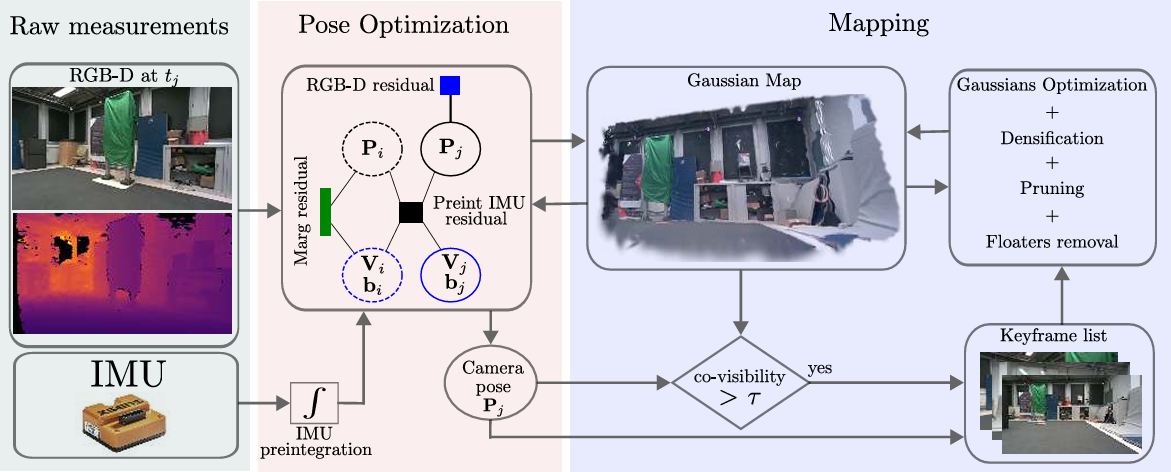
\includegraphics[width=0.75\linewidth]{../imagenes_marco_teorico/pipeline_vigs_fusion.png}
    \caption{Pipeline del paper VIGS-Fusion. Los keyframes son elegidos cuando la co-visibilidad con el frame actual supera un umbral $\tau$. En la optimización de la pose obtienen residuos de marginalización, de RGB-D y de la IMU.}
    \label{fig:pipeline_vigs_fusion}
\end{figure}

Ahora, veamos el método presentado por el paper.

\subsection{Optimización de la pose}

El estado a tiempo $k$ se define como

\begin{equation}
    x_k = [\mb{P}_k, \mb{V}_k, \mb{b}_a^k, \mb{b}_g^k]
\end{equation}

con $\mb{P}_k \in SE(3)$ representando la traslación $\mb{p}_k \in \mathbb{R}^3$ y la rotación $\mb{R}_k \in SO(3)$; $\mb{V}_k$ la velocidad; $\mb{b}_a^k$ y $\mb{b}_g^k$ los sesgos del acelerómetro y giróscopo, respectivamente.

Para optimizar, se define una función de costo general que combina los residuos de RGB-D, de IMU y de marginalización:

\begin{equation}
C(\mb{x}_k) = r_{RGB-D} + r_{IMU} + r_{Marg}
\end{equation}

Para la minimización se utilizó Levenberg-Marquadt, con una aproximación del segundo orden $r_{RGB-D}$, en contraste con los métodos del estado del arte que utilizaban descenso del gradiente de primer orden.

Para calcular el Jacobiano respecto de la pose $\mb{P}_k$, se planteó desde el álgebra de Lie, teniendo en cuenta que $\mb{P}_k \in SE(3)$ induce una representación $\xi_k = [\rho, \omega]^T \in \mathfrak{se}(3)$ con $\rho \in \mathbb{R}^3$ la traslación y $\omega \in \mathbb{R}^3$ la rotación. En este caso, la actualización se hace con perturbación a izquierda, porque el paper premultiplica el incremento al estado:

\begin{equation}
\mb{P}_{k+1} = \exp(\delta \xi)\,\mb{P}_k = \delta \xi \oplus_{\mathrm{izq}} \mb{P}_k
\end{equation}

Esta convención se conserva aquí para mantener la formulación original del método, pero queda explícito que la perturbación es a izquierda.

\subsection{Residuo RGB-D}
Este residuo se compone del residuo fotométrico, que es la diferencia entre el color observado y el renderizado, $r_{photo} = RGB(x) - C(x)$, y el residuo geométrico, que es la diferencia entre la profundidad observada y la renderizada, $r_{geo} = D(x) - d(x)$. Para calcular la profundidad renderizada $d(x)$ se consideró la mediana de las profundidades de las gaussianas calculadas con \ref{profundidad_gaussianas}.

\begin{equation}
r_{RGB-D} = r_{photo} + r_{geo}
\end{equation}

En la literatura, se utiliza descenso del gradiente computando el Jacobiano a partir del modelo de color y profundidad, requiriendo muchos parámetros para poder diferenciar la suma de gaussianas pesadas. En este paper, se determinó un cambio que consiste en usar las derivadas de la imagen observada en el espacio bidimensional. Para obtener los Jacobianos se diferenciaron el color observado $RGB(x)$ y la profundidad $D(x)$.

\subsubsection{Jacobiano del error fotométrico}

\begin{equation}
\mb{J}_{\xi_c}^{r_{photo}} = \frac{\mc{D}r_{photo}}{\mc{D}\xi_c} = 
\frac{\mc{D}(RGB(x) - C(x))}{\mc{D}\xi_c} = \frac{\mc{D}RGB(x)}{\mc{D}\xi_c}
\label{jacobiano_error_fotometrico}
\end{equation}

Utilizando los gradientes de la imagen observada, se aplicó la regla de la cadena

\begin{equation}
\frac{\mc{D}RGB(x)}{\mc{D}\xi_c} = \frac{\mc{D}RGB(x)}{\mc{D}\mb{u}} 
\frac{\mc{D}\mb{u}}{\mc{D}\mb{u}_c} \frac{\mc{D}\mb{u}_c}{\mc{D}\xi_c}
\end{equation}

donde $\mb{u}(u_x, u_y)$ es la ubicación del píxel en el plano bidimensional, y $\mb{u}_c$ su ubicación en el espacio tridimensional en el sistema de referencia de la cámara.

A partir de esta descomposición, se tienen los siguientes términos:

\begin{itemize}
    \item 
    El gradiente de la imagen respecto de cada color y dirección:
    \begin{equation}
    \frac{\mc{D}RGB(x)}{\mc{D}\mb{u}} =
    \begin{bmatrix}
        g_{u_x}^R & g_{u_x}^G & g_{u_x}^B\\
        g_{u_y}^R & g_{u_y}^G & g_{u_y}^B
    \end{bmatrix} ^T
    \end{equation}
    donde $g_{u_a}^b$ representa el gradiente en la dirección $a$ del canal $b$.
    
    \item 
    El Jacobiano de la proyección de la cámara deducido en \ref{jacobiano_proyeccion_camara}.
    $\frac{\mc{D}\mb{u}}{\mc{D}\mb{u}_c} = \mb{J}_c$

    \item 
    El Jacobiano de los puntos respecto de un movimiento en la pose
    \begin{equation}
    \frac{\mc{D}\mb{u}_c}{\mc{D}\xi_c}
    \end{equation}
    Para encontrar una fórmula cerrada, \cite{Matsuki2024GaussianSplattingSLAM} utilizó la derivación en la variante. Así, la perturbación $\delta \xi_c$, descompuesta en su traslación $\rho'$ y su rotación $\omega'$ induce la acción sobre el punto
    
    \begin{equation}
    \mb{u}_c' = (\mb{I} + [\omega']_X) \mb{u}_c + \rho
    \end{equation}

    por lo que la perturbación lleva a la diferencia

    \begin{equation}
    \delta\mu_c = \mu_c' - \mu_c = \rho + [\omega]_X \mu_c = \rho - [\mu_c]_X \,\,\omega
    \end{equation}

    Luego, podemos expresar el Jacobiano como

    \begin{equation}
    \frac{\mc{D}\mb{u}_c}{\mc{D}\xi_c} = 
    \begin{bmatrix}
        \mb{I} & -[\mb{u}_c]_X
    \end{bmatrix}
    \label{jacobiano_puntos_pose}
    \end{equation}
\end{itemize}

\subsubsection{Jacobiano del error geométrico}

\begin{equation}
    \mb{J}_{\xi_c}^{r_{geo}} = \frac{\mc{D}(D(x) - d(x))}{\mc{D}\xi_c} = \frac{\mc{D}D(x)}{\mc{D}\xi_c}
\end{equation}

Mediante la regla de la cadena,

\begin{equation}
    \frac{\mc{D}D(x)}{\mc{D}\xi_c} = \frac{\mc{D}D(\mb{x})}{\mc{D}\mb{u}_c}
    \frac{\mc{D}\mb{u}_c}{\mc{D}\xi_c}
\end{equation}

De nuevo, tenemos una descomposición con los términos:

\begin{itemize}
    \item 
    La dirección del rayo. Despejando en \ref{proyeccion_pinhole}, surge que
    \begin{equation}
    \frac{\mc{D}D(\mb{x})}{\mc{D}\mb{u}_c} = r = 
    \begin{bmatrix}
        \frac{u_x - c_x}{f_x} \\
        \frac{u_y - c_y}{f_y}
    \end{bmatrix}
    \end{equation}

    \item 
    El Jacobiano de los puntos respecto de un movimiento en la pose, que ya calculamos en \ref{jacobiano_puntos_pose}
\end{itemize}



\subsubsection{Resultados para $r_{RGB-D}$}

Al plantear los residuos como una matriz de la forma

\begin{equation}
    \mb{r}_{RGB-D} =
    \begin{bmatrix}
        \mb{r}_{photo} \\
        \mb{r}_{geo}
    \end{bmatrix}
\end{equation}

se expresa el Jacobiano completo

\begin{equation}
    \mb{J}_{\xi_c}^{r_{RGB-D}} =
    \begin{bmatrix}
        \mb{J}_{\xi_c}^{r_{photo}} \\
        \mb{J}_{\xi_c}^{r_{geo}}
    \end{bmatrix}
\end{equation}

Luego, para poder usar Levenberg-Marquadt se tienen las expresiones

\begin{equation}
    {\mb{J}_{\xi_c}^{r_{RGB-D}}}^T \mb{J}_{\xi_c}^{r_{RGB-D}} =
    {\mb{J}_{\xi_c}^{r_{photo}}}^T \mb{J}_{\xi_c}^{r_{photo}} +
    {\mb{J}_{\xi_c}^{r_{geo}}}^T \mb{J}_{\xi_c}^{r_{geo}}
\end{equation}
    
\begin{equation}
    {\mb{J}_{\xi_c}^{r_{RGB-D}}}^T \mb{r}_{RGB-D} =
    {\mb{J}_{\xi_c}^{r_{photo}}}^T \mb{r}_{photo} +
    {\mb{J}_{\xi_c}^{r_{geo}}}^T \mb{r}_{geo}
\end{equation}


%%%%%%%%%%%%%%%%%%%%%%%%%

\subsection{Residuo IMU}

El estado del sistema en el instante $k$ se define como

\begin{equation}
\mathbf{x}_k =
\left(
\mathbf{p}_k,
\mathbf{q}_k,
\mathbf{v}_k,
\mathbf{b}_{a_k},
\mathbf{b}_{g_k}
\right)
\end{equation}

donde $\mathbf{p}_k$ es la posición, $\mathbf{q}_k$ la orientación, $\mathbf{v}_k$ la velocidad y $\mathbf{b}_{a_k},\mathbf{b}_{g_k}$ representan los sesgos del acelerómetro y el giroscopio respectivamente.

Entre dos fotogramas consecutivos $i$ y $j$, las mediciones de la IMU se preintegran obteniendo las cantidades

\begin{equation}
(\Delta \mathbf{p}_{ij}, \Delta \mathbf{v}_{ij}, \Delta \mathbf{q}_{ij})
\end{equation}

que representan los cambios relativos de posición, velocidad y orientación expresados en el sistema de referencia del instante $i$.

Siguiendo la formulación de la preintegración en variedades, la predicción del estado en el instante $j$ a partir del estado en $i$ puede escribirse como

\begin{align}
\mathbf{p}_j &=
\mathbf{p}_i
+
\mathbf{v}_i \Delta t
+
\frac12 \mathbf{g} \Delta t^2
+
\mathbf{R}_i
\Delta \mathbf{p}_{ij}
\\
\mathbf{v}_j &=
\mathbf{v}_i
+
\mathbf{g}\Delta t
+
\mathbf{R}_i
\Delta \mathbf{v}_{ij}
\\
\mathbf{q}_j &=
\mathbf{q}_i
\otimes
\Delta \mathbf{q}_{ij}
\end{align}

donde $\mathbf{R}_i$ es la matriz de rotación asociada al cuaternión $\mathbf{q}_i$.

El residuo IMU compara la predicción obtenida mediante estas ecuaciones con el estado estimado por el optimizador. Se define entonces como

\begin{equation}
\mathbf{r}_{IMU}
=
\begin{bmatrix}
\mathbf{r}_p \\
\mathbf{r}_q \\
\mathbf{r}_v \\
\mathbf{r}_{ba} \\
\mathbf{r}_{bg}
\end{bmatrix}
\end{equation}

donde cada componente corresponde a un error en posición, orientación, velocidad y sesgos.

El residuo de posición se define como

\begin{equation}
\mathbf{r}_p =
\mathbf{R}_i^\top
\left(
\mathbf{p}_j
-
\mathbf{p}_i
-
\mathbf{v}_i \Delta t
-
\frac12 \mathbf{g}\Delta t^2
\right)
-
\Delta \mathbf{p}_{ij}
\end{equation}

El residuo de velocidad se expresa como

\begin{equation}
\mathbf{r}_v =
\mathbf{R}_i^\top
\left(
\mathbf{v}_j
-
\mathbf{v}_i
-
\mathbf{g}\Delta t
\right)
-
\Delta \mathbf{v}_{ij}
\end{equation}

Para la orientación se utiliza la diferencia de cuaterniones en el grupo $SO(3)$

\begin{equation}
\mathbf{r}_q =
(\mathbf{q}_i^{-1}\mathbf{q}_j)
\ominus
\Delta\mathbf{q}_{ij}
\end{equation}

Utilizando la parametrización mínima del error rotacional en $SO(3)$, este término puede escribirse explícitamente como

\begin{equation}
\mathbf{r}_q =
2\,\mathrm{vec}
\left(
\Delta \mathbf{q}_{ij}^{-1}
(\mathbf{q}_i^{-1}\mathbf{q}_j)
\right).
\end{equation}

donde $\mathrm{vec}(\cdot)$ extrae la parte vectorial del cuaternión.

Los residuos asociados a los sesgos se definen como

\begin{align}
\mathbf{r}_{ba} &= \mathbf{b}_{a_j} - \mathbf{b}_{a_i} \\
\mathbf{r}_{bg} &= \mathbf{b}_{g_j} - \mathbf{b}_{g_i}
\end{align}

Para resolver el problema mediante optimización no lineal, el residuo se linealiza alrededor de una estimación actual $\tilde{\mathbf{x}}$.

\begin{equation}
\mathbf{r}_{IMU}(\mathbf{x})
\approx
\mathbf{r}_{IMU}(\tilde{\mathbf{x}})
+
\mathbf{J}
\delta \mathbf{x}
\end{equation}

donde

\begin{equation}
\mathbf{J}
=
\frac{\partial \mathbf{r}_{IMU}}{\partial \mathbf{x}}
\end{equation}

es el Jacobiano del residuo respecto al estado.

Por ejemplo, derivando el residuo de posición respecto a $\mathbf{p}_i$ se obtiene

\begin{equation}
\frac{\partial \mathbf{r}_p}{\partial \mathbf{p}_i}
=
-\mathbf{R}_i^\top
\end{equation}

mientras que respecto a $\mathbf{p}_j$

\begin{equation}
\frac{\partial \mathbf{r}_p}{\partial \mathbf{p}_j}
=
\mathbf{R}_i^\top
\end{equation}

y respecto a la velocidad inicial

\begin{equation}
\frac{\partial \mathbf{r}_p}{\partial \mathbf{v}_i}
=
-\mathbf{R}_i^\top \Delta t
\end{equation}

Las derivadas respecto a la orientación utilizan la aproximación de primer orden de la rotación

\begin{equation}
\mathbf{R}(\delta \boldsymbol{\theta})
\approx
\mathbf{I}
+
[\delta \boldsymbol{\theta}]_\times
\end{equation}

Finalmente, los residuos se ponderan mediante la matriz de información de la medición

\begin{equation}
\|r\|^2 =
\mathbf{r}_{IMU}^\top
\mathbf{W}
\mathbf{r}_{IMU}
\end{equation}

donde $\mathbf{W}=\boldsymbol{\Sigma}^{-1}$ es la inversa de la covarianza de la preintegración.



%%%%%%%%%%%%%%%%%%%%%%%%%%%%%%%%%%%%%%%%%%%%%%%
\subsection{Residuo de marginalización}

Al obtener nuevos datos, el sistema estima un nuevo estado $\mathbf{x}_k$. 
Para mantener el problema de optimización computacionalmente manejable, se utiliza 
una estrategia de \textit{ventana deslizante}, donde los estados más antiguos se eliminan 
de la optimización. Sin embargo, eliminar directamente dichos estados implicaría perder 
la información contenida en las mediciones asociadas a ellos. 

Para evitar esta pérdida de información, se realiza un proceso de \textit{marginalización}, 
mediante el cual las variables antiguas se eliminan del problema pero su información se 
condensa en un nuevo factor que actúa como un prior sobre las variables restantes.

Sea el vector completo de variables del problema

\begin{equation}
\mathbf{x} =
\begin{bmatrix}
\mathbf{x}_m \\
\mathbf{x}_r
\end{bmatrix}
\end{equation}

donde

\begin{itemize}
\item $\mathbf{x}_m$ representa las variables que se desean marginalizar (estados antiguos),
\item $\mathbf{x}_r$ representa las variables que permanecerán en la optimización.
\end{itemize}

El problema de mínimos cuadrados puede escribirse como

\begin{equation}
\min_{\mathbf{x}}
\|\mathbf{r}(\mathbf{x})\|^2
\end{equation}

donde $\mathbf{r}(\mathbf{x})$ es el vector de residuos del sistema.

Linealizando alrededor de una estimación actual $\tilde{\mathbf{x}}$ se obtiene

\begin{equation}
\mathbf{r}(\mathbf{x})
\approx
\mathbf{r}_0 + \mathbf{J}\delta\mathbf{x}
\end{equation}

donde

\begin{equation}
\delta\mathbf{x} =
\mathbf{x} \ominus \tilde{\mathbf{x}}
\end{equation}

y $\mathbf{J}$ es el Jacobiano del residuo.

El sistema normal asociado al problema de mínimos cuadrados es

\begin{equation}
\mathbf{A}\delta\mathbf{x} = \mathbf{b}
\end{equation}

con

\begin{align}
\mathbf{A} &= \mathbf{J}^\top \mathbf{J} \\
\mathbf{b} &= \mathbf{J}^\top \mathbf{r}_0
\end{align}

Separando las variables a marginalizar y las variables restantes, la matriz 
$\mathbf{A}$ puede escribirse como

\begin{equation}
\mathbf{A} =
\begin{bmatrix}
\mathbf{A}_{mm} & \mathbf{A}_{mr} \\
\mathbf{A}_{rm} & \mathbf{A}_{rr}
\end{bmatrix}
\end{equation}

y el vector $\mathbf{b}$ como

\begin{equation}
\mathbf{b} =
\begin{bmatrix}
\mathbf{b}_m \\
\mathbf{b}_r
\end{bmatrix}.
\end{equation}

Para eliminar las variables $\mathbf{x}_m$ se aplica el complemento de Schur, 
obteniéndose un nuevo sistema reducido

\begin{align}
\mathbf{A}^\ast &= 
\mathbf{A}_{rr} -
\mathbf{A}_{rm}
\mathbf{A}_{mm}^{-1}
\mathbf{A}_{mr}
\\
\mathbf{b}^\ast &=
\mathbf{b}_r -
\mathbf{A}_{rm}
\mathbf{A}_{mm}^{-1}
\mathbf{b}_m
\end{align}

que depende únicamente de las variables restantes $\mathbf{x}_r$.

Este sistema reducido define un nuevo factor que encapsula la información de las 
variables marginalizadas.

Para integrarlo nuevamente en el optimizador, se busca una factorización de la forma

\begin{equation}
\mathbf{A}^\ast =
\mathbf{J}_{marg}^\top
\mathbf{J}_{marg}
\end{equation}

donde $\mathbf{J}_{marg}$ es el jacobiano del nuevo factor de marginalización.

En la implementación, esta factorización se obtiene mediante descomposición espectral

\begin{equation}
\mathbf{A}^\ast =
\mathbf{V}
\mathbf{\Lambda}
\mathbf{V}^\top
\end{equation}

de donde se define

\begin{equation}
\mathbf{J}_{marg} =
\sqrt{\mathbf{\Lambda}}
\mathbf{V}^\top .
\end{equation}

El residuo asociado al factor de marginalización se define entonces como

\begin{equation}
\mathbf{r}_{marg}(\mathbf{x}_r)
=
\mathbf{r}_0
+
\mathbf{J}_{marg}
\delta\mathbf{x}_r
\end{equation}

donde

\begin{equation}
\mathbf{r}_0 =
\mathbf{J}_{marg}^{-T}
\mathbf{b}^\ast .
\end{equation}

Finalmente, el incremento de estado utilizado en la evaluación del residuo es

\begin{equation}
\delta\mathbf{x}_r =
\mathbf{x}_r \ominus \mathbf{x}_r^0
\end{equation}

donde $\mathbf{x}_r^0$ es el punto de linearización almacenado en el momento de 
realizar la marginalización.

En el caso de variables definidas en $SE(3)$, el incremento se calcula en el 
espacio tangente. Para una pose representada por posición $\mathbf{p}$ y 
cuaternión $\mathbf{q}$ se utiliza

\begin{equation}
\delta\mathbf{x} =
\begin{bmatrix}
\mathbf{p}-\mathbf{p}_0 \\
2\,\mathrm{vec}
\left(
\mathbf{q}_0^{-1}\mathbf{q}
\right)
\end{bmatrix}.
\end{equation}

De esta manera, el factor de marginalización actúa como un prior gaussiano 
sobre las variables restantes, preservando la información de los estados 
eliminados mientras se mantiene constante el tamaño del problema de optimización.




%%%%%%%%%%%%%%%%%%%%%%%%%%%%%%%%%%%%%%%%%%%%%%%%%%%%%%%%%%%%%%%%%%%%%%%%%%%%%%%%

\subsection{Función de costo para gaussianas}

En este trabajo se utiliza una función de costo compuesta por tres términos, análoga a la de otros trabajos como RAD-GS \cite{radgs}:

\begin{equation}
\mathcal{L} = \mathcal{L}_{\text{rgb}} + w_{\text{depth}} \mathcal{L}_{\text{depth}} + w_{\text{dist}} \mathcal{L}_{\text{dist}} + \lambda_{\text{iso}} \mathcal{L}_{\text{iso}}
\end{equation}

donde:

\paragraph{Término fotométrico ($\mathcal{L}_{\text{rgb}}$):}
Mide la diferencia cuadrática entre el color renderizado y el observado en cada píxel:
\begin{equation}
\mathcal{L}_{\text{rgb}} = \sum_{p} \frac{1}{2}\|C(p) - C^*(p)\|_2^2
\end{equation}
con $C(p) = \sum_n T_n \alpha_n c_n$ el color renderizado mediante alpha-blending ordenado en profundidad.

\paragraph{Término de profundidad mediana ($\mathcal{L}_{\text{depth}}$):}
Penaliza la diferencia entre la profundidad renderizada en el punto mediano de transmitancia (cuando $T$ cruza 0.5) y la profundidad observada:
\begin{equation}
\mathcal{L}_{\text{depth}} = \sum_{p} \frac{w_{\text{depth}}}{2}\, \mathbf{1}_{\text{med}}(p)\, \big(D_{\text{med}}(p) - D^*(p)\big)^2
\end{equation}
donde $\mathbf{1}_{\text{med}}(p)$ es un indicador que vale 1 en el splat donde la transmitancia cruza 0.5, y la profundidad en ese punto es:
\begin{equation}
D_{\text{med}}(p) = z_n + \hat{p}_n \cdot (p - \mu_n^{2D})
\end{equation}
con $\hat{p}_n$ el vector que codifica cómo varía la profundidad con el desplazamiento en imagen.

\paragraph{Término de distorsión de profundidad ($\mathcal{L}_{\text{dist}}$):}
Regulariza la consistencia entre la profundidad de cada splat y la profundidad mediana acumulada, pesando por la contribución de cada gaussiana:
\begin{equation}
\mathcal{L}_{\text{dist}} = \sum_{p,n} \frac{w_{\text{dist}}}{2}\, \alpha_n(p)\,T_n(p)\, \big(d_n(p)-D_{\text{med}}(p)\big)^2
\end{equation}
donde $d_n(p) = z_n + \hat{p}_n \cdot (p - \mu_n^{2D})$ es la profundidad de la gaussiana $n$ en el píxel $p$.

\paragraph{Término de regularización isotrópica ($\mathcal{L}_{\text{iso}}$):}

Penaliza que las gaussianas sean muy anisótropas (muy alargadas en una dirección), favoreciendo formas más esféricas:

\begin{equation}
\mathcal{L}_{\text{iso}} = \sum_{n} \lambda_{\text{iso}}\sum_{i} (s_{n,i} - \bar{s}_n)^2
\end{equation}
donde $s_{n,i}$ son las componentes de escala de la gaussiana $n$ y $\bar{s}_n = (s_{n,x} + s_{n,y} + s_{n,z})/3$.

Esta formulación permite balancear la fidelidad fotométrica con restricciones geométricas provenientes de sensores RGB-D, crucial para mantener una reconstrucción métrica consistente en SLAM visual.




\subsection{Gradientes}

Dada la función de costo, ahora podemos calcular los gradientes respecto de los parámetros de las gaussianas. Para esto, VIGS-Fusion plantea cálculo sobre las imágenes proyectadas, simplificando el costo computacional de las derivadas. A continuación, se detallan los cálculos para cada tipo de parámetro.

\subsubsection{Gradiente de color}

El color se forma a partir del alpha-blending de los splats bidimensionales. Por tanto,

\begin{equation}
C = \sum_n T_n \alpha_n c_n
\end{equation}

con $T_n$ la transmitancia, $\alpha_n$ la opacidad y $c_n$ el color de la gaussiana $n$ en orden de profundidad back-to-front.

Luego, tenemos que, sea $e = C - C_{obs}$ tal que $L = \frac{1}{2}||e||^2$ sea la función de pérdida,

\begin{equation}
    \frac{\partial L}{\partial c_n} = 
    \frac{\partial L}{\partial C} \frac{\partial C}{\partial c_n} =
    e (T_n\alpha_n)
\end{equation}

Ahora, para poder extenderlo a la gaussiana tridimensional, no es necesario realizar ningún cambio, ya que el color no se perturba al proyectar. Podemos simplemente usar

\begin{equation}
    \frac{\partial L}{\partial c_n^{3d}} = \frac{\partial L}{\partial c_n^{2d}}
\end{equation}



\subsubsection{Gradiente de opacidad}

Para la opacidad $\alpha_n$, tenemos que la misma influye activamente en el término correspondiente a la gaussiana $n$, y en todas las posteriores a partir del alpha-blending, pues

\begin{equation}
T_n = \prod_{k<n}(1-\alpha_k) 
\end{equation}

Al derivar, tenemos tanto el término propio de color $T_n \alpha_n c_n$ como todos los términos posteriores. Como el término propio es lineal en $\alpha_n$, la derivada es simplemente $T_n c_n$. Por otro lado, para un $m>n$ fijo,

\begin{equation}
\frac{\partial T_m}{\partial \alpha_n} = - \frac{T_m}{1 - \alpha_n}
\end{equation}

Luego,

\begin{equation}
    \frac{\partial C}{\partial \alpha_n} = T_nc_n - \frac{1}{1-\alpha_n} \sum_{m>n}T_m\alpha_mc_m
    = T_n c_n - \frac{C - C_{\leq n}}{1-\alpha_n}
\end{equation}

con $C_{\leq n}$ el color acumulado hasta n.

Finalmente,

\begin{equation}
    \frac{\partial L}{\partial \alpha_n} = 
    \frac{\partial L}{\partial C} \frac{\partial C}{\partial \alpha_n} =
    e (T_n c_n - \frac{C - C_{\leq n}}{1-\alpha_n})
\end{equation}


\subsubsection{Gradiente de la media}

Para calcular el gradiente de la media $\mu_{3D}$, lo separamos en:

\begin{equation}
    \frac{\partial L}{\partial \mu_{3D}} =
    \frac{\partial L}{\partial \mu_{2D}} \frac{\partial \mu_{2D}}{\partial \mu_{3D}}
    + \frac{\partial L}{\partial z} \frac{\partial z}{\partial \mu_{3D}}
    + \frac{\partial L}{\partial \Sigma'} \frac{\partial \Sigma'}{\partial \mu_{3D}}
\end{equation}

Ahora, deducimos cada término

\paragraph{Media bidimensional}

Sea $\mb{J}$ el jacobiano de la proyección,

\begin{equation}
    \frac{\partial \mu_{2D}}{\partial \mu_{3D}} = \mb{J}
\end{equation}

Para el factor restante, observamos que la media bidimensional influye en la
pérdida a través del peso gaussiano proyectado. Sea

\begin{equation}
G(x) =
\exp\!\left(
-\frac{1}{2} (x-\mu_{2D})^T \Sigma'^{-1} (x-\mu_{2D})
\right),
\end{equation}

y sea $\alpha = \sigma G$ la opacidad efectiva del splat en el píxel.
Entonces,

\begin{equation}
\frac{\partial \alpha}{\partial \mu_{2D}}
=
\alpha \, \Sigma'^{-1}(x-\mu_{2D}).
\end{equation}

Aplicando regla de la cadena,

\begin{equation}
\frac{\partial L}{\partial \mu_{2D}}
=
\frac{\partial L}{\partial \alpha}
\frac{\partial \alpha}{\partial \mu_{2D}}
=
\frac{\partial L}{\partial \alpha}
\alpha
\Sigma'^{-1}(x-\mu_{2D}).
\end{equation}

\paragraph{Profundidad}

La coordenada de profundidad es simplemente la tercera componente de la media en el sistema de referencia de la cámara:

\begin{equation}
    z = \mu_{3D,z}
\end{equation}

Por lo tanto,

\begin{equation}
    \frac{\partial z}{\partial \mu_{3D}} =
    \begin{bmatrix}
        0 & 0 & 1
    \end{bmatrix}
\end{equation}

y el término correspondiente del gradiente queda

\begin{equation}
    \frac{\partial L}{\partial z}
    \frac{\partial z}{\partial \mu_{3D}}
    =
    \frac{\partial L}{\partial z}
    \begin{bmatrix}
        0 & 0 & 1
    \end{bmatrix}.
\end{equation}

Para obtener $\frac{\partial \mathcal{L}}{\partial z}$, observamos que la profundidad aparece en dos lugares de la función de costo:

\paragraph{Deducción del gradiente del término de profundidad mediana}

El término de profundidad mediana es:
\begin{equation}
\mathcal{L}_{\text{depth}} = \sum_{p} \frac{w_{\text{depth}}}{2}\, \mathbf{1}_{\text{med}}(p)\, \big(D_{\text{med}}(p) - D^*(p)\big)^2
\end{equation}

Recordando que $D_{\text{med}}(p) = z_n + \hat{p}_n \cdot (p - \mu_n^{2D})$ para la gaussiana $n$ donde $T$ cruza 0.5, derivamos respecto a $z_n$:

\begin{equation}
\begin{split}
\frac{\partial \mathcal{L}_{\text{depth}}}{\partial z_n} &= \sum_{p} w_{\text{depth}} \, \mathbf{1}_{\text{med}}(p) \, \big(D_{\text{med}}(p) - D^*(p)\big) \frac{\partial D_{\text{med}}(p)}{\partial z_n} \\
&= \sum_{p} w_{\text{depth}} \, \mathbf{1}_{\text{med}}(p) \, \big(D_{\text{med}}(p) - D^*(p)\big) \cdot 1 \\
&= w_{\text{depth}} \, \mathbf{1}_{\text{med}}(n) \, (D_{\text{med}} - D^*)
\end{split}
\end{equation}

donde el indicador $\mathbf{1}_{\text{med}}(n)$ vale 1 únicamente en el píxel donde la gaussiana $n$ cruza $T=0.5$, y $\frac{\partial D_{\text{med}}}{\partial z_n} = 1$ ya que $D_{\text{med}}$ depende linealmente de $z_n$.

\paragraph{Deducción del gradiente del término de distorsión}

El término de distorsión es:
\begin{equation}
\mathcal{L}_{\text{dist}} = \sum_{p,n} \frac{w_{\text{dist}}}{2}\, \alpha_n(p)\,T_n(p)\, \big(d_n(p)-D_{\text{med}}(p)\big)^2
\end{equation}

Derivando respecto a $z_n$ (la profundidad de la gaussiana $n$):

\begin{equation}
\begin{split}
\frac{\partial \mathcal{L}_{\text{dist}}}{\partial z_n} &= \sum_{p} w_{\text{dist}} \, \alpha_n(p)\,T_n(p)\, \big(d_n(p) - D_{\text{med}}(p)\big) \frac{\partial d_n(p)}{\partial z_n} \\
&= \sum_{p} w_{\text{dist}} \, \alpha_n(p) \, T_n(p) \, (d_n(p) - D_{\text{med}}(p)) \cdot 1 \\
&= \sum_p w_{\text{dist}} \, \alpha_n(p) \, T_n(p) \, (d_n(p) - D_{\text{med}}(p))
\end{split}
\end{equation}

donde usamos que $d_n(p) = z_n + \hat{p}_n \cdot (p - \mu_n^{2D})$, de modo que $\frac{\partial d_n(p)}{\partial z_n} = 1$. 


En esta derivación, $D_{\text{med}}(p)$ se trata como constante respecto a $z_n$ mediante un \textit{stop-gradient}, es decir, considerando nulo el gradiente. Esto es correcto porque: (1) si $n$ no es el splat mediano en el píxel $p$, entonces $D_{\text{med}}(p)$ efectivamente depende de otro splat diferente, no de $z_n$; (2) si $n$ \emph{es} el splat mediano, ambas derivadas $\frac{\partial d_n}{\partial z_n} = 1$ y $\frac{\partial D_{\text{med}}}{\partial z_n} = 1$ se cancelarían, resultando en contribución nula.


\paragraph{Gradiente total respecto a la profundidad}

Por lo tanto, el gradiente total respecto a la profundidad es:
\begin{equation}
\frac{\partial \mathcal{L}}{\partial z_n} = \frac{\partial \mathcal{L}_{\text{depth}}}{\partial z_n} + \frac{\partial \mathcal{L}_{\text{dist}}}{\partial z_n}
\end{equation}

Este gradiente se acumula sobre todos los píxeles donde la gaussiana $n$ tiene contribución significativa, aplicándose el primer término solo en el píxel mediano y el segundo en todos los píxeles.



\paragraph{Covarianza proyectada}

Recordemos que la covarianza proyectada se describe en términos de la covarianza como

\begin{equation}
    \Sigma' = \mb{J} \, \Sigma \, \mb{J}^T
\end{equation}

donde $\mb{J}$ depende de la media 3D a través de la proyección perspectiva.

Luego, al derivar respecto de la media

\begin{equation}
    \frac{\partial \Sigma'}{\partial \mu_{3D}} = 
    \frac{\partial (\mb{J} \Sigma \mb{J}^T)}{\partial \mu_{3D}} =
    \frac{\partial \mb{J}}{\partial \mu_{3D}} \Sigma \mb{J} ^T 
    + \mb{J} \Sigma \frac{\partial \mb{J}^T}{\partial \mu_{3D}}
\end{equation}

Como consideramos la proyección afín local para todas las cuentas, se considera que el jacobiano es constante, dando lugar a que

\begin{equation}
    \frac{\partial \mb{J}}{\partial \mu_{3D}} \approx 0
\end{equation}

Luego, este término se anula.



\subsubsection{Gradientes respecto a Covarianza, Escala y Rotación}

Recordemos la parametrización de la covarianza en el sistema de referencia del mundo:

\begin{equation}
\Sigma = R S^2 R^T
\end{equation}

donde:
\begin{itemize}
    \item $R \in SO(3)$ es la matriz de rotación (obtenida del cuaternión),
    \item $S = \mathrm{diag}(s_x, s_y, s_z)$ contiene las escalas.
\end{itemize}

En esta formulación, la covarianza proyectada $\Sigma'$ resulta

\begin{equation}
\Sigma = \mb{T} \Sigma_{3D} \mb{T}^T
\end{equation}

donde:

\begin{equation}
T = J W
\end{equation}

y:
\begin{itemize}
    \item $J$ es el Jacobiano de proyección perspectiva,
    \item $W$ es la rotación cámara-mundo.
\end{itemize}

En lugar de optimizar directamente la covarianza 3D $\Sigma$, se parametrizan la rotación y la escala, para asegurarse de que la matriz resultante simétrica definida positiva, además de que brinda un sentido geométrico más sólido. Sin embargo, para calcular estos gradientes, es necesario, también, calcular el de la covarianza.

\paragraph{Gradiente respecto a la covarianza 3D}

Aplicando la regla de la cadena:

\begin{equation}
\frac{\partial \mathcal{L}}{\partial \Sigma_{3D}}
=
\mb{T}^T
\frac{\partial \mathcal{L}}{\partial \Sigma'}
\mb{T}
\end{equation}

Para obtener $\frac{\partial \mathcal{L}}{\partial \Sigma'}$, notamos que la covarianza 2D afecta a la pérdida a través de la forma gaussiana y, por tanto, de la opacidad $\alpha_n(p) = \sigma_n \exp(-\frac{1}{2}\delta^T \Sigma'^{-1} \delta)$, donde $\delta = p - \mu_n^{2D}$.

Usamos la identidad para la derivada de una inversa:
\begin{equation}
\frac{\partial F}{\partial A}
=
- A^{-T}
\frac{\partial F}{\partial A^{-1}}
A^{-T}
\end{equation}

Luego:
\begin{equation}
\frac{\partial \mathcal{L}}{\partial \Sigma'} = - \Sigma'^{-1} \frac{\partial \mathcal{L}}{\partial \Sigma'^{-1}} \Sigma'^{-1}
\end{equation}

Observando que:
\begin{equation}
\frac{\partial G}{\partial \Sigma'^{-1}} = -\frac{1}{2} G \, \delta \delta^T
\end{equation}

y

\begin{equation}
    \frac{\partial \alpha}{\partial G} = \sigma
\end{equation}

Aplicando la regla de la cadena, cadena:
\begin{equation}
\frac{\partial \mathcal{L}}{\partial \Sigma'^{-1}} = \frac{\partial \mathcal{L}}{\partial \alpha} \frac{\partial \alpha}{\partial G} \frac{\partial G}{\partial \Sigma'^{-1}} = 
-\frac{1}{2} \frac{\partial \mathcal{L}}{\partial \alpha} \, \sigma\, G\, \delta \delta^T
= -\frac{1}{2} \frac{\partial \mathcal{L}}{\partial \alpha} \, \alpha\, \delta \delta^T
\end{equation}

Este último paso surge de que $\alpha = \sigma G$

Este gradiente se acumula sobre todos los píxeles donde la gaussiana contribuye.



\paragraph{Gradiente respecto a la escala}

Sea $M \coloneq \mb{R} \mb{S}$, entonces

\begin{equation}
\Sigma_{3D} = M M^T
\end{equation}

El gradiente respecto a $M$ es:

\begin{equation}
\frac{\partial \mathcal{L}}{\partial M}
= 2 \frac{\partial \mathcal{L}}{\partial \Sigma} M
\end{equation}

Luego, por definición de $M$, el gradiente para la escala es

\begin{equation}
\frac{\partial \mathcal{L}}{\partial s_i}
=
R_{:,i}^T
\left(
\frac{\partial \mathcal{L}}{\partial M}
\right)_{:,i}
\end{equation}

Es posible expresar las escalas en logaritmo, en tal caso:

\begin{equation}
s_i = e^{\tilde{s}_i}
\end{equation}

entonces:

\begin{equation}
\frac{\partial \mathcal{L}}{\partial \tilde{s}_i}
=
\frac{1}{s_i}
\frac{\partial \mathcal{L}}{\partial s_i}
\end{equation}

\paragraph{Regularización isotrópica}

Para mantener una relación entre las escalas, se introduce un término de pérdida que depende solo de la escala:

\begin{equation}
\mathcal{L}_{iso}
=
\lambda_{iso}
\sum_i (s_i - \bar{s})^2
\end{equation}

donde:

\begin{equation}
\bar{s} = \frac{s_x + s_y + s_z}{3}
\end{equation}

Su gradiente es:

\begin{equation}
\frac{\partial \mathcal{L}_{iso}}{\partial s}
=
\frac{\lambda_{iso}}{3}
\begin{bmatrix}
2\Delta_x - \Delta_y - \Delta_z \\
-\Delta_x + 2\Delta_y - \Delta_z \\
-\Delta_x - \Delta_y + 2\Delta_z
\end{bmatrix}
\end{equation}

donde $\Delta_i = s_i - \bar{s}$.


\paragraph{Gradiente respecto a la rotación}

Recordemos que la covarianza se parametriza como

Aplicando regla de la cadena sobre $M = RS$,

\begin{equation}
\frac{\partial \mathcal{L}}{\partial R}
=
\frac{\partial \mathcal{L}}{\partial M} S .
\end{equation}

Sin embargo, $R \in SO(3)$, por lo que su gradiente debe proyectarse al
espacio tangente del grupo. Las variaciones admisibles de $R$ pueden
escribirse como

\begin{equation}
dR = R[\delta\theta]_\times ,
\end{equation}

Utilizando esta parametrización y propiedades del producto traza, se obtiene
que el gradiente respecto al vector de rotación viene dado por

\begin{equation}
\frac{\partial \mathcal{L}}{\partial \theta}
=
-
\sum_{i=1}^{3}
R_{:,i}
\times
\left(
\frac{\partial \mathcal{L}}{\partial R}
\right)_{:,i}.
\end{equation}

\subsubsection{Peso por relevancia}

En la práctica, es conveniente mantener proporcionalmente más estáticas a las gaussianas que participan en más píxeles, y menos a las que no. Debido a esto, se define un factor que depende de la cantidad de observaciones $n$ de la gaussiana

\begin{equation}
    \eta = \eta(n) \coloneq \frac{1}{5 + n}
\end{equation}

El mismo se multiplica al gradiente real antes de pasarlo al algoritmo de optimización. Notemos que, a mayor $n$, menor $\eta$, por lo que el gradiente será más bajo y tenderá a modificarse menos en la iteración del optimizador.